\subsection{Use Cases}
\label{UseCases}
For at sikre at vi laver et program, der fungerer som ønsket, har vi opstillet flere use cases for systemet.
Disse use cases er blevet udledt på baggrund af møder med Psykolog Nords ledelse, og ved brug af de fire basis funktioner for persistens: create, read, update og delete (CRUD), på objekt- og domænemodelen.
Derudover har vi også identificeret primæraktørene og deres mål, og sikret at vores use cases opfylder målene.

Vores primæraktører og deres mål er:

\begin{itemize}
    \item Bookingansvarlig
        \begin{itemize}
            \item Se aftaler
            \item Book aftale
            \item Ændr aftale
            \item Aflys aftale
        \end{itemize}
    \item Psykolog
        \begin{itemize}
            \item Ajourfør kundes journal
        \end{itemize}
    \item Kunde
        \begin{itemize}
            \item Se og betal fakturaer
            \item Book aftale
            \item Ændr aftale
            \item Aflys aftale
        \end{itemize}

\end{itemize}

Det er f.eks. vigtigt at skelne mellem at booke en ny aftale, ændre den og aflyse den, da det er tre forskellige funktionaliteter i systemet.

\begin{figure}[ht]
	\centering
  		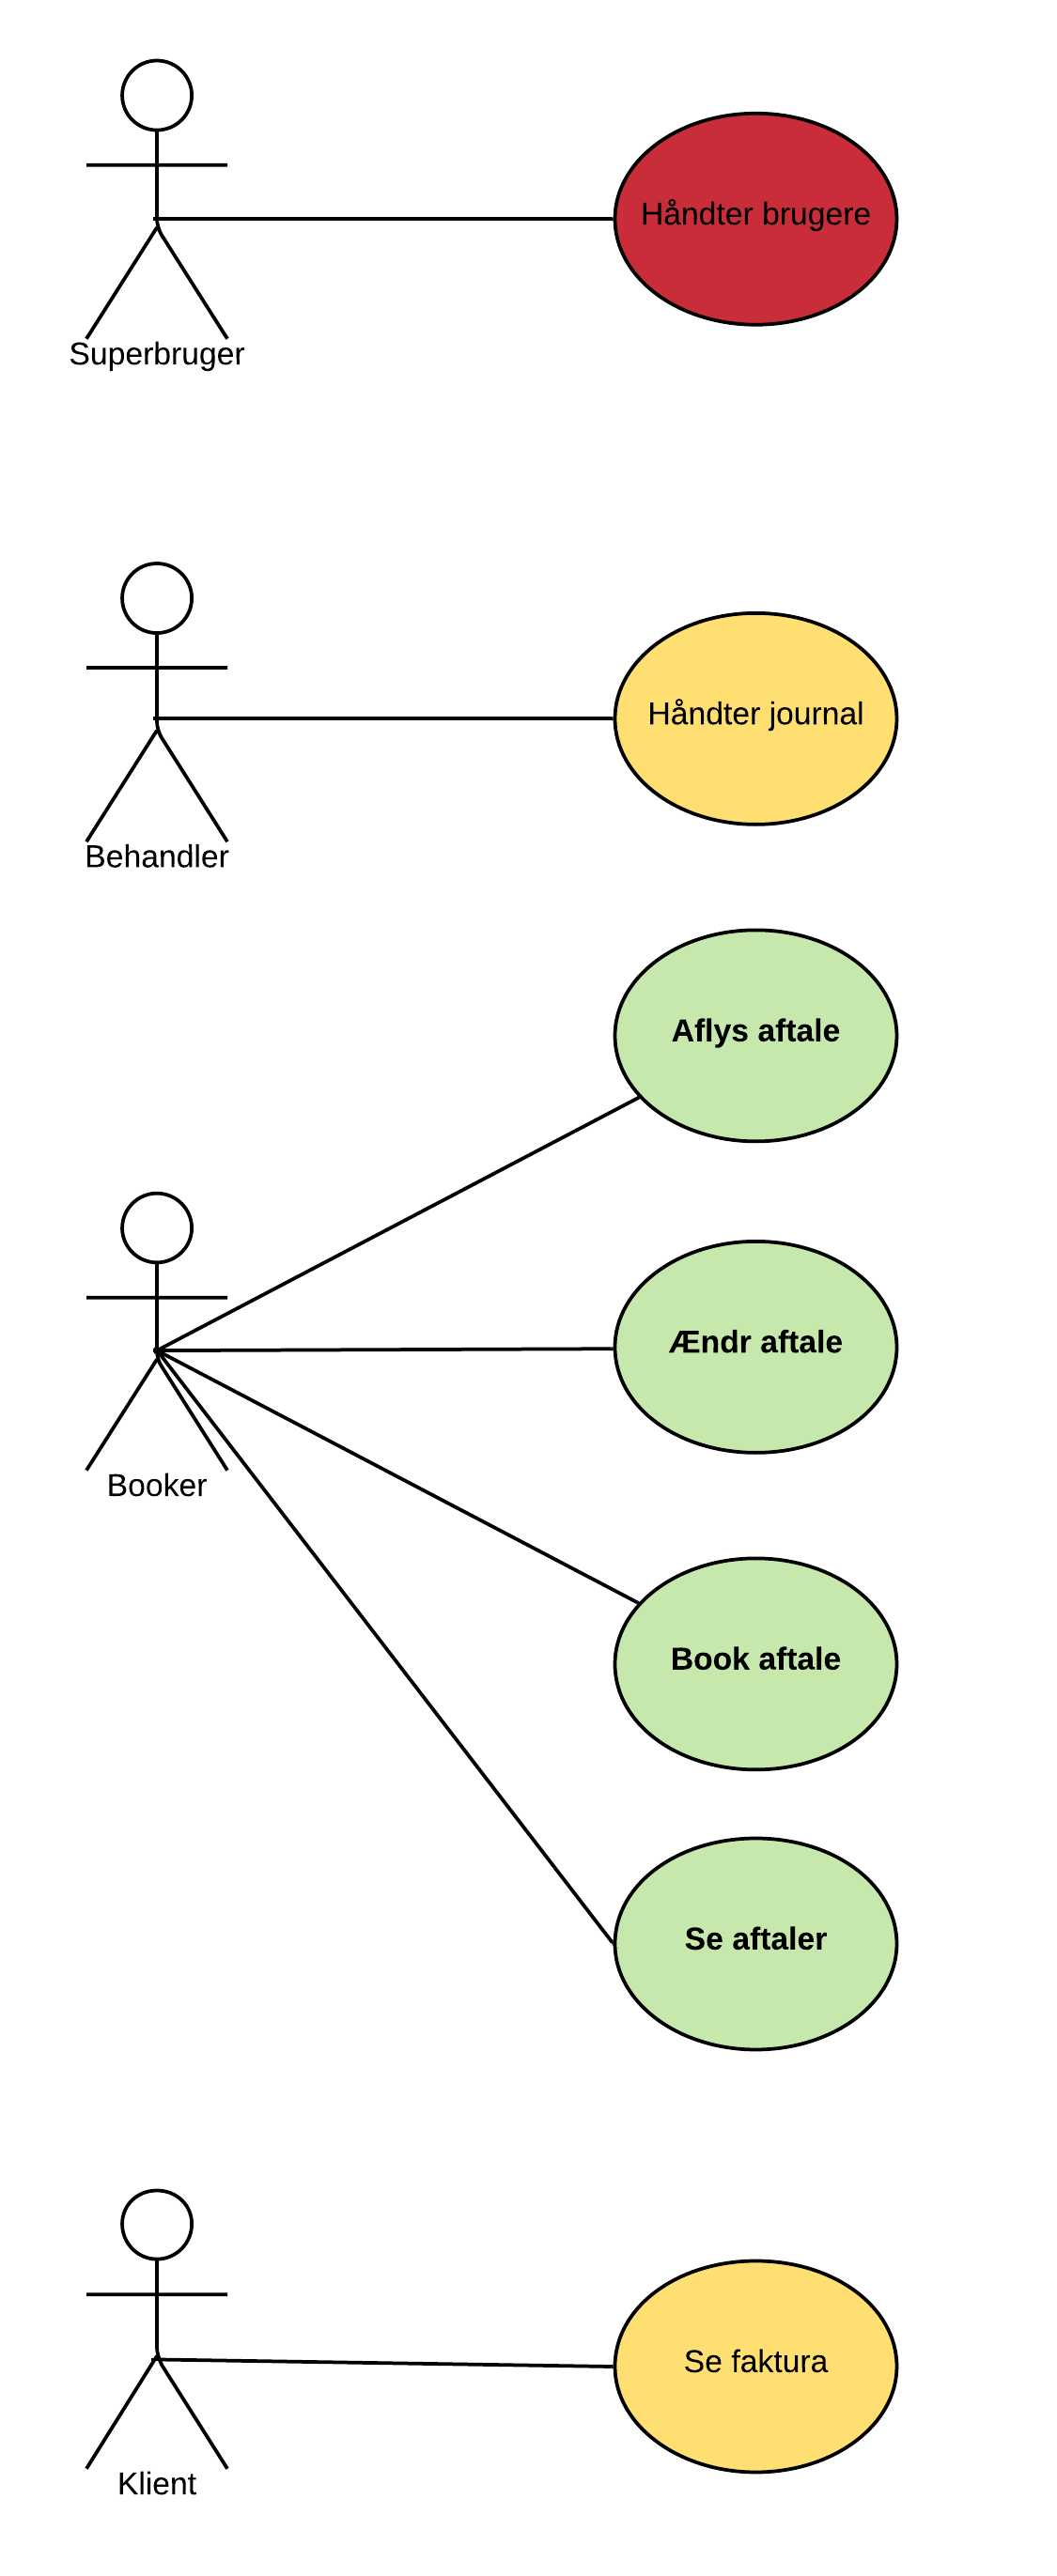
\includegraphics[scale=0.75]{UseCaseDiagram.png}
  \caption{Use Case diagram.}
  \label{fig:UseCaseDiagram}
\end{figure}

På figur \ref{fig:UseCaseDiagram} kan man se alle de use cases vi fandt frem til.
Uses casesne er blevet markeret med farver, der repræsenterer deres prioritering under projektforløbet: de grønne var dem, som Psykolog Nord først ønskede implementeret og derefter gul.
I følgende afsnit kan man så findes vores use cases beskrevet mere detaljeret. 

To personer deltager i en aftale: en kunde og en psykolog.

\subsubsection{Use Case: Book aftale}\label{usecase:bookaftale}
{\setlength{\parindent}{0cm}
\textbf{Scope:} Bookingsystem for Psykolog Nord

\textbf{Primær Aktør:} Bookingansvarlig

\textbf{Hovedscenarie (succes):} Booking af ny aftale

Den bookingansvarlige ønsker at booke en aftale.
Hvis den involverede kunde ikke har brugt PsykologNord før, oprettes kunden i systemet.
Kunden vælger aftaletype og der bookes en ny aftale, hvor både kunden og psykologen har tid. 
Aftalen bookes og kunde og psykolog notificeres.

\textbf{Primær Aktør:} Kunde og bookingansvarlig

\textbf{Alternativt scenarie (succes):} Kontakt PsykologNord for at booke en aftale

En kunde ønsker at booke en aftale, og kontakter derfor PsykologNord.
En bookingansvarlig booker aftalen som i hovedscenariet.

\textbf{Primær Aktør:} Kunde

\textbf{Alternativt scenarie (succes):} Vælge Parterapi som aftale

En kunde ønsker at booke en parterapi aftale.
Hvis den involverede kunde ikke har brugt PsykologNord før, oprettes kunden i systemet.
Kunden vælger aftaletype, og indtaster den anden kundes informationer, og den anden kunde oprettes også i systemet.
Der bookes en ny aftale, hvor både kunden og psykologen har tid. 
Aftalen bookes, begge kunder og psykologen notificeres.
}

For at se resten af use casene se bilag \ref{bilag:UseCases}, på side \pageref{bilag:UseCases}
